% Frontend
\chapter{Aplikacje mobilne}
\label{part:applications}

% Brak przecinka przed zamiast
Oparcie rozwiązania o Firebase pozwoliło znacznie uprościć część backendową, która sprowadza się jedynie do opisanego w kolejnym rozdziale projektu Firebase. Dodało to jednak wiele odpowiedzialności ciążących na stronie klienckiej. Ponadto decyzja o stworzeniu dwóch aplikacji mobilnych zamiast jednej przyczynia się do dalszej jej komplikacji. Z wymienionych powodów opracowanie aplikacji mobilnych stanowiło dominującą część całego projektu i zastosowane wewnątrz nich rozwiązania wymagały głębokiego przemyślenia.

% Brak przecinka przed zamiast
% Oparcie projektu o Firebase pozwala znacznie uprościć lub wręcz usunąć część backendową, lecz dodaje więcej odpowiedzialności ciążących na stronie klienckiej. Należy równocześnie mieć na uwadze wcześniejsze założenie, co do stworzenia dwóch aplikacji mobilnych zamiast jednej. Z wymienionych powodów implementacja części klienckiej stanowi dominującą część całego projektu i dlatego zastosowane wewnątrz niej rozwiązania wymagają głębokiego przemyślenia.

\section{Architektura}

Odpowiednio dobrana architektura umożliwia płynny rozwój aplikacji, nawet, przy bardzo dużej i ciągle rosnącej bazie kodu. Jest to również najważniejszy element wpływający na solidność oraz możliwość testowania.

Jedną z główny cech, jaką dobra architektura powinna się charakteryzować, jest jasne i precyzyjne określenie odpowiedzialności posiadanych przez poszczególne części programu. Podział aplikacji na jak najbardziej niezależne sekcje jest sugerowany przez regułę projektowania zwaną skrótowo SoC (ang. Separation of Concerns). Zgodnie z nią każda z nich powinna zajmować się innym problemem, pracować z innymi informacjami.

Architekturą, która doskonale spełnia wymienione wymagania, jest trójwarstwowa architektura rekomendowana przez Google dla aplikacji mobilnych. Składają się na nią warstwy prezentacji, domenowa oraz danych, z których każda pełni inne funkcje. Zostały one przedstawione na rysunku \ref{fig:ca-warstwy}.

\begin{figure}[ht]
  \centering
  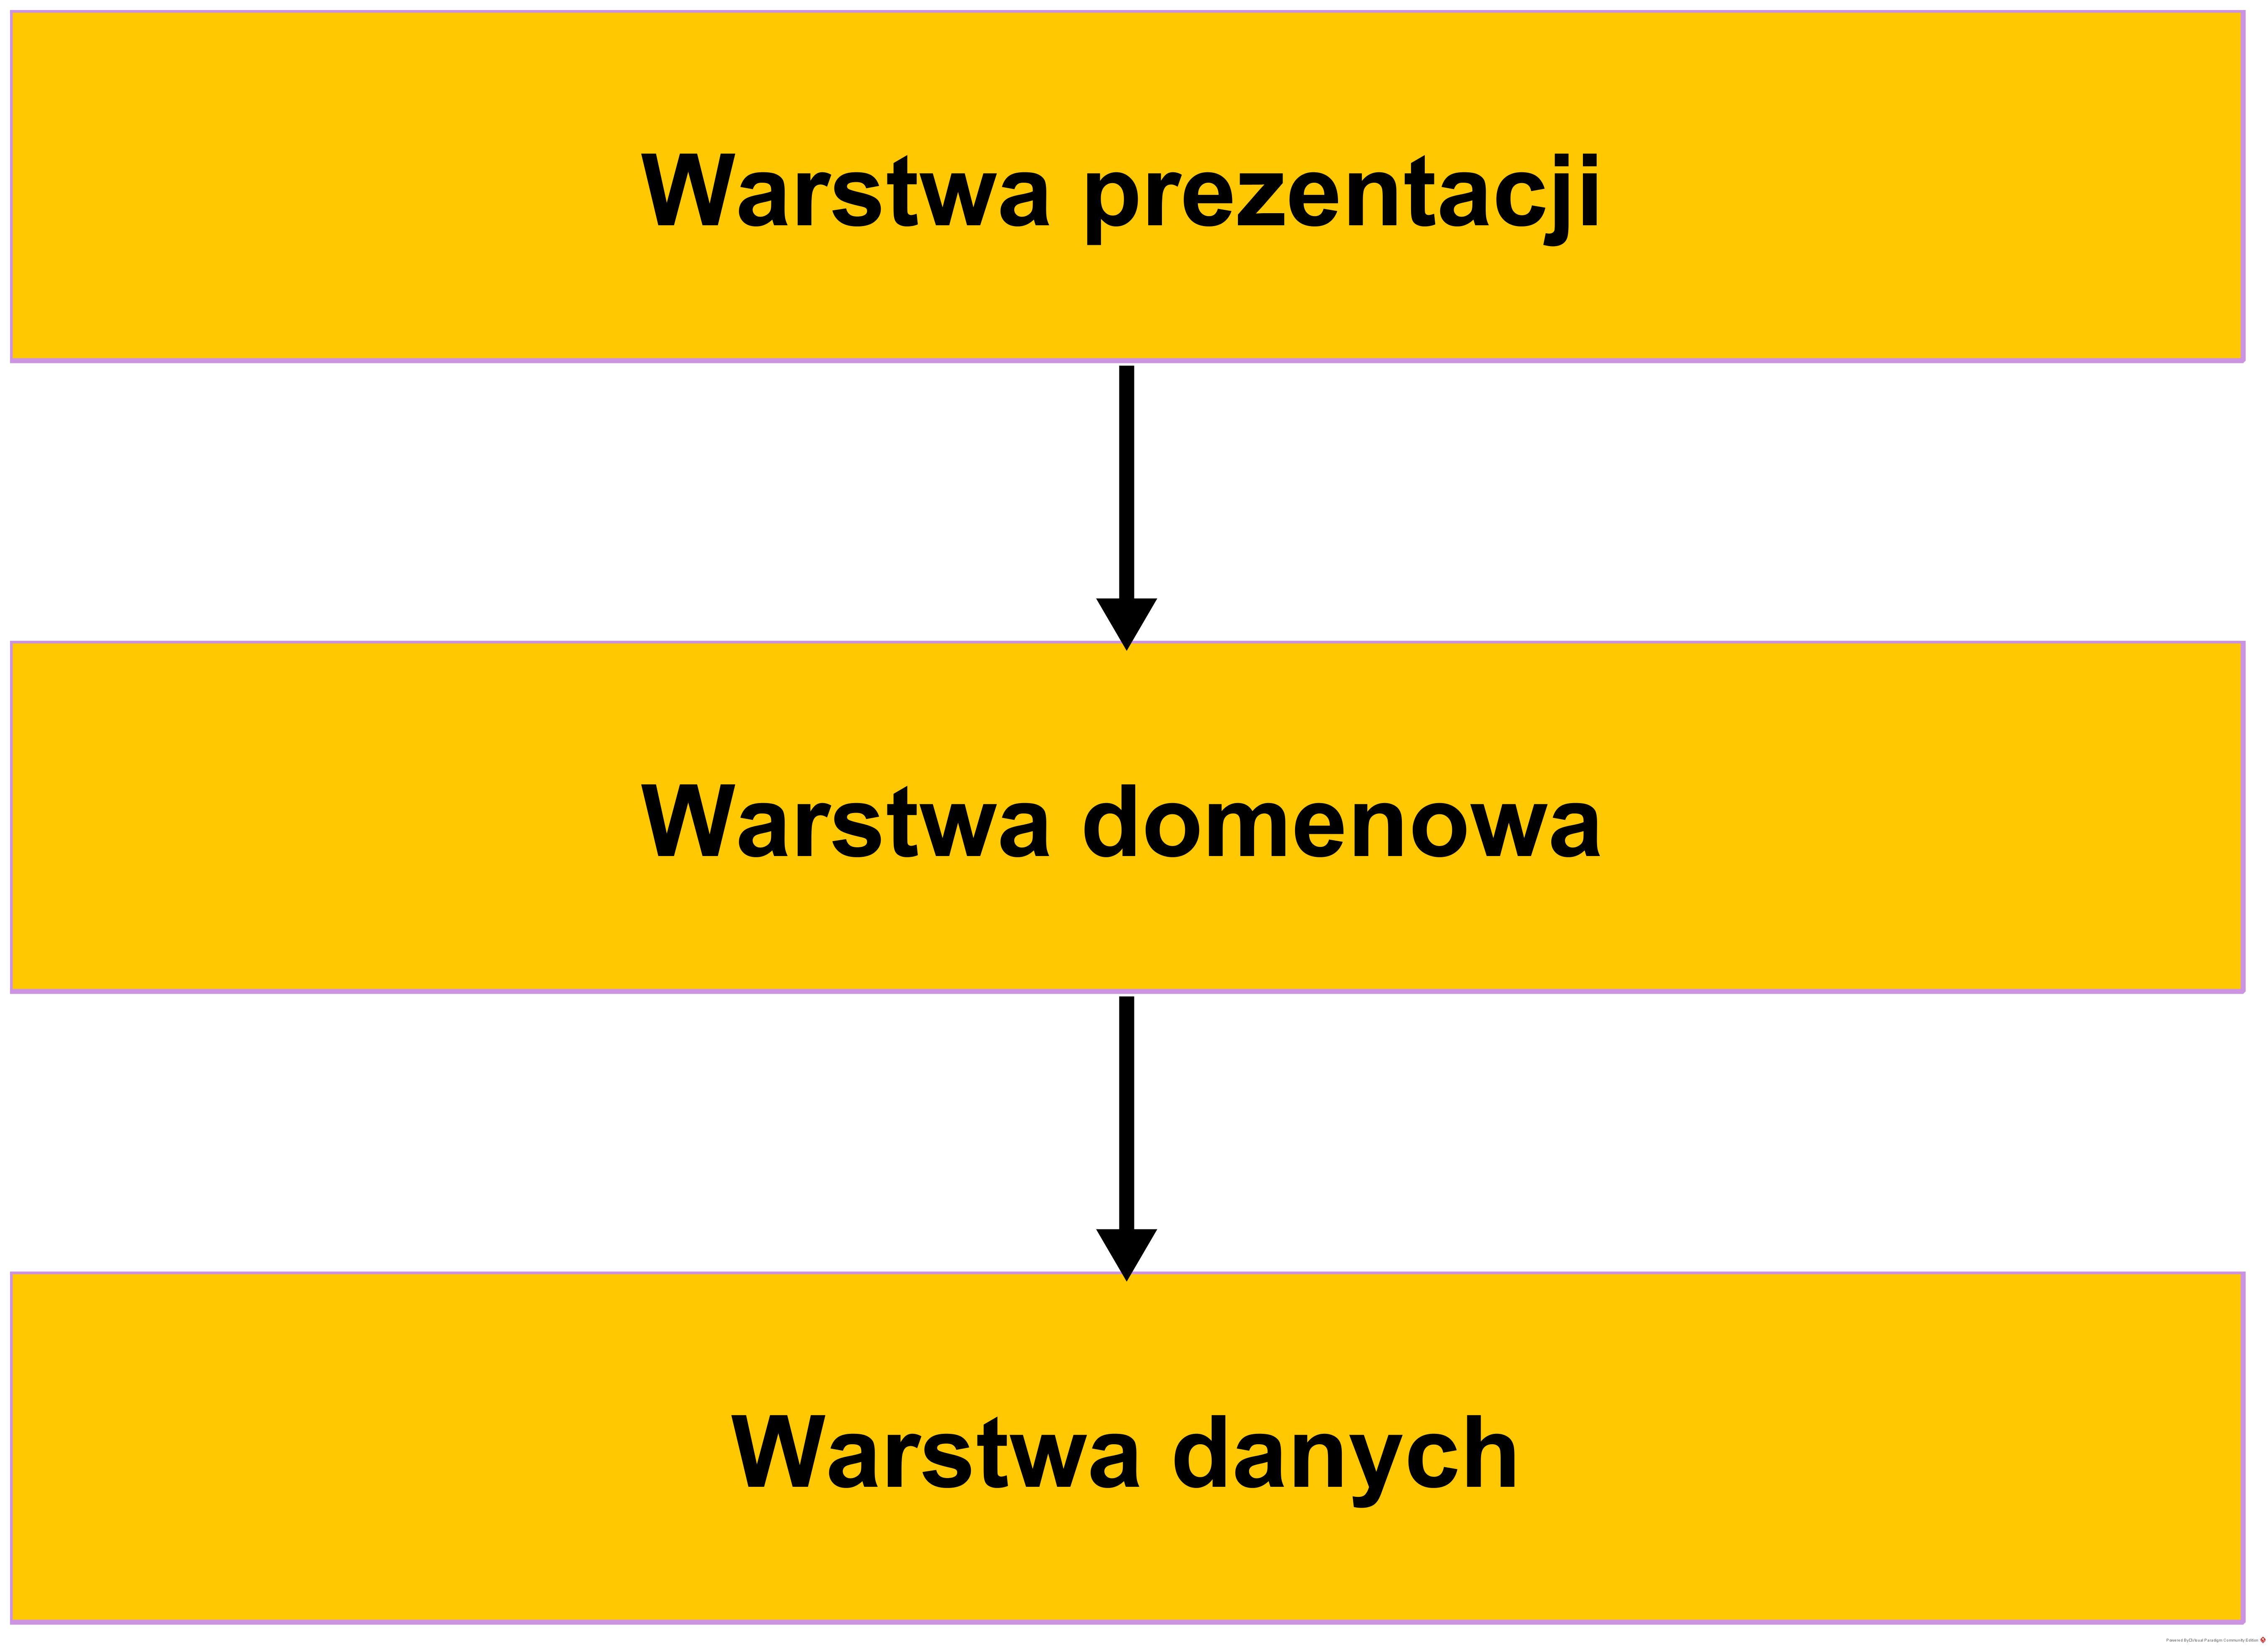
\includegraphics[width=0.8\linewidth]{images/arch_layers.png}
  \caption{Schemat warstw aplikacji}
  \label{fig:ca-warstwy}
\end{figure}

Warstwa prezentacji jest odpowiedzialna za przekazywanie informacji użytkownikowi, aktualizowanie ich, jeżeli ulegają zmianie oraz przechwytywanie podejmowanych przez niego akcji, takich jak kliknięcia czy przesunięcia po ekranie.

Warstwa danych zapewnia dostęp do informacji przechowywanych w różnego rodzaju trwałych magazynach. Zawiera w sobie logikę dotyczącą sposobu pobierania, tworzenia, modyfikowania oraz usuwania różnych obiektów.

Celem warstwy domenowej jest przechowywanie logiki biznesowej. Jest ona zawarta w postaci tak zwanych przypadków użycia. Każdy z nich odpowiada za inny scenariusz. Przykładowe przypadki użycia, które zostały stworzone to dodanie zlecenia, wysłanie wiadomości, pobranie dostępnych zleceń czy wylogowanie. Ich obecność umożliwia zamknięcie skomplikowanej logiki oraz wielokrotne użycie. Warstwa ta zawiera również klasy określające obiekty domenowe, czyli te najistotniejsze, takie jak zlecenie, wiadomość, wykonawca czy klient.

Zgodnie ze wskazówkami dotyczącymi architektury, znajdującymi się w dokumentacji platformy Android, obecność warstwy domenowej nie jest zawsze konieczna. W przypadku, gdy aspekt ponownego wykorzystania nie jest kluczowy oraz logika biznesowa jest prosta, to może ona prowadzić do powstania większej ilości kodu, bez wprowadzenia dodatkowych korzyści. Biorąc jednak pod uwagę, że tworzone będą dwie aplikacje, które z pewnością będą współdzieliły część logiki biznesowej stwierdzono, że wielokrotne użycie jest istotną kwestią i zdecydowano się tę warstwę wykorzystać.

% Na warstwę domenową składają się dwa typy elementów: modele domenowe oraz przypadki użycia. Modele domenowe to klasy reprezentujące pojęcia występująca w dziedzinie rozważanego problemu, np. zlecenie, oferta, wykonawca, klient czy wiadomość. Przypadki użycia są to natomiast operacje związane z tą dziedzina, np. dodanie zlecenia, akceptacja oferty, wysłanie wiadomości, pobranie dostępnych zleceń czy wylogowanie.

% Bardzo ważny jest kierunek zależności istniejących pomiędzy tymi warstwami. Zarówno warstwa prezentacji jak i warstwa danych jest zależna od warstwy domenowej. Umożliwia to skupienie się na dziedzinie aplikacji, która stanowi jej rdzeń. Ten kierunek umożliwia również dokonywanie zmian w warstwie prezentacji i warstwie danych bez większego wpływu na warstwy pozostałe.

% Aby zrozumieć przydatność przypadków użycia należy wiedzieć, że wykonywane przez nie operacje mogą być dość skomplikowane. Przykładem jest przypadek użycia polegający na pobraniu informacji o zleceniu z punktu widzenia aktualnie zalogowanego wykonawcy. W pierwszej kolejności, korzystając z warstwy danych, pobiera on identyfikator aktualnego użytkownika. Następnie pobiera podstawowe informacje o zleceniu i korzystając z wcześniej pobranego identyfikatora użytkownika, pobiera status zlecenia. Ostatecznie łączy te wyniki do postaci pojedynczego obiektu domenowego, który zwraca. W ten sposób udaje się zamknąć wewnątrz niego dużą złożoność, a warstwa prezentacji, która go wywołuje jest świadoma jedynie parametrów oraz zwracanej przez niego wartości, co jest ważne tym bardziej, że jeden przypadek może być wykorzystywany w kilku miejscach.

% Wykorzystanie przypadków użycia usprawniło również obsługę błędów. Operacje wykonywane w ich ramach mogą bowiem często zakończyć się błędem. Czasami niepowodzenie jednej z operacji cząstkowych oznacza niepowodzenia całego przypadku użycia, a czasem nie. 

% Owszem, zdarza się, że przypadki użycia bezpośrednio odpowiadają metodom znajdującym się w warstwie danych, jak ma to miejsce w przypadku dodawania oceny, gdzie na przypadek użycia składa się tylko jedno wywołanie.

\section{Warstwa prezentacji}
\label{wzorzec-mvvm}

W ramach warstwy prezentacji wykorzystany został wzorzec MVVM (ang. Model-View-ViewModel), który umożliwia czyste i jasne oddzielenie kwestii związanych z interfejsem użytkownika od warstwy domenowej. Stosowanie go jest wspierane przez platformę Android poprzez dostarczanie gotowych komponentów, które to ułatwiają. Dostępna jest między innymi klasa ViewModel, która umożliwia zachowanie w niej stanu aplikacji podczas zmian konfiguracji, takich jak obroty urządzenia.

Tak jak sugeruje nazwa, na wzorzec MVVM składają się komponenty: Model, View oraz ViewModel. Zostały one przedstawione wraz z relacjami pomiędzy sobą na rysunku \ref{fig:mvvm}.

\begin{figure}[ht!]
  \centering
  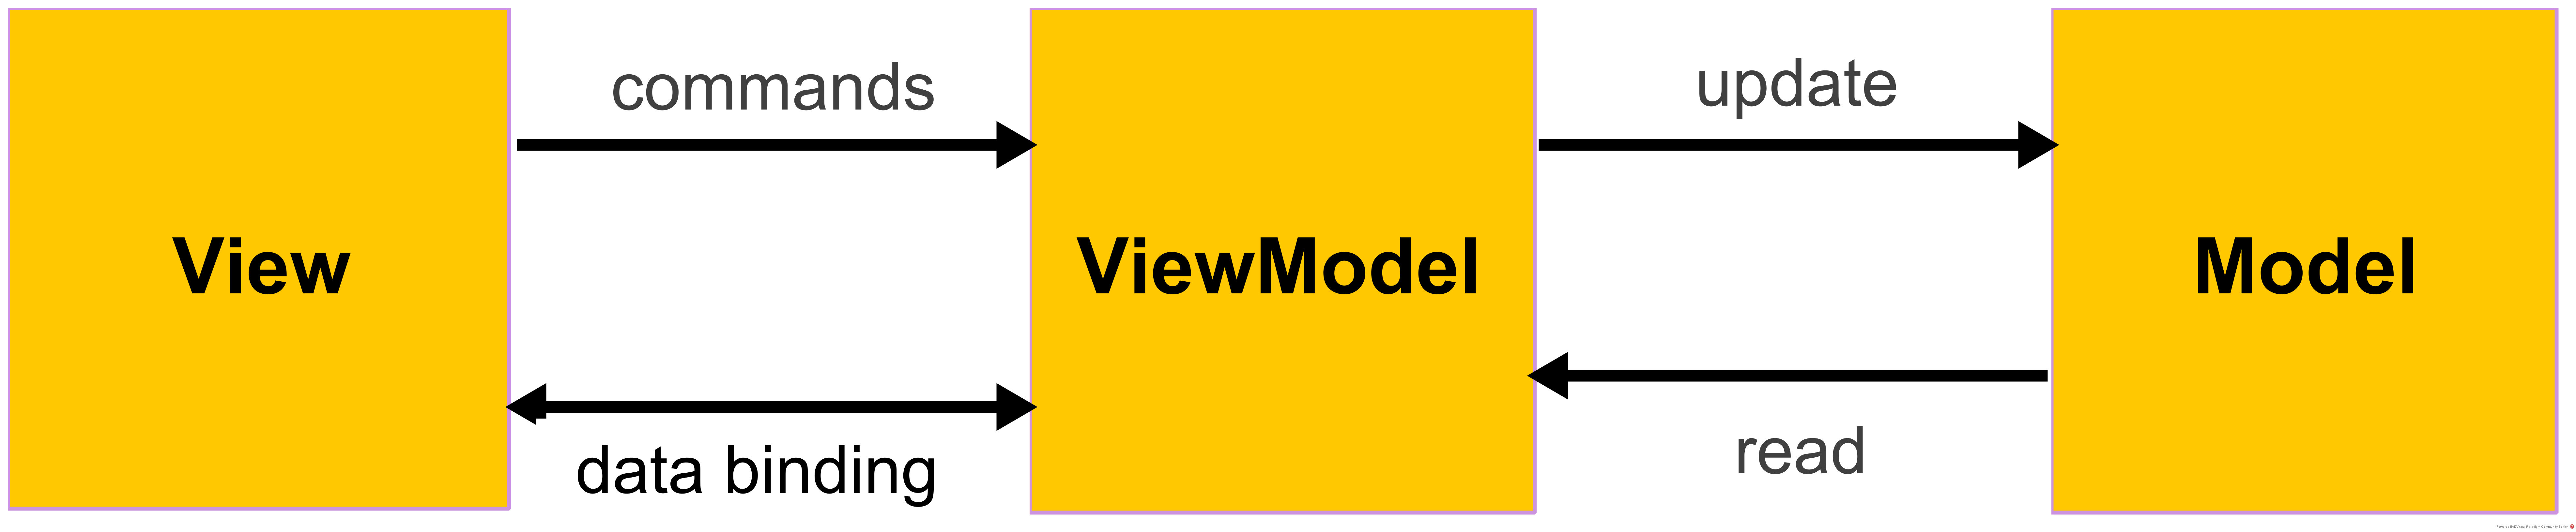
\includegraphics[width=\linewidth]{images/mvvm_general.png}
  \caption{Schemat komponentów wzorca MVVM i ich relacji}
  \label{fig:mvvm}
\end{figure}

View jest widokiem, czyli tym co widzi użytkownik oraz z czym wchodzi w interakcję. W przygotowanym rozwiązaniu wszystkimi widokami są fragmenty, które stanowią reużywalną część interfejsu użytkownika, więc doskonale się do tego nadają. Komponent model odnosi się z kolei do modelu biznesowego i oznacza całą warstwę domenową, na którą składają się przypadki użycia i modele domenowe. Ostatnim komponentem jest ViewModel, który pełni ważna funkcję polegającą na połączeniu dwóch pozostałych. W ten sposób umożliwia ich niezależny rozwój. Ponadto przechowuje stan.

Interakcja komponentu ViewModel z modelem biznesowym sprowadza się do wykonywania przypadków użycia, za pomocą których model może zostać zmodyfikowany lub mogą zostać z niego odczytane dane.
Widok nie może robić tego bezpośrednio, więc jeśli potrzebuje wejść w interakcję z modelem, to jedynie za pośrednictwem ViewModel.

Pomiędzy komponentami View oraz ViewModel wykorzystywana jest technika zwana data binding, która w ogólnym znaczeniu polega na zapewnieniu synchronizacji ze sobą dwóch źródeł danych. Dzięki niej każda zmiana stanu komponentu ViewModel może zostać natychmiastowo odzwierciedlona w widoku. Możliwe są także wiązania dwukierunkowe, zapewniające synchronizację w obie strony. Korzystanie z tej techniki jest proste, z uwagi na dostępną w ramach Android Jetpack biblioteki, która ją wspiera.

%Wykonuje przypadki użycia z warstwy domenowej i po ewentualnym przetworzeniu udostępnia ich wyniki widokowi, by mógł je wyświetlić.



% Komunikacja ViewModel z View zachodzi poprzez mechanizm subskrypcji udostępniany przez obiekty LiveData, będące częścią platformy Android. Gdy widok zasupskrybuje taką wartość, to będzie powiadamiany o wszystkich jej późniejszych zmianach.

%W celu usprawnienia komunikacji pomiędzy View oraz ViewModel wykorzystana została biblioteka Data Binding

% \begin{figure}[ht!]
%   \centering
%   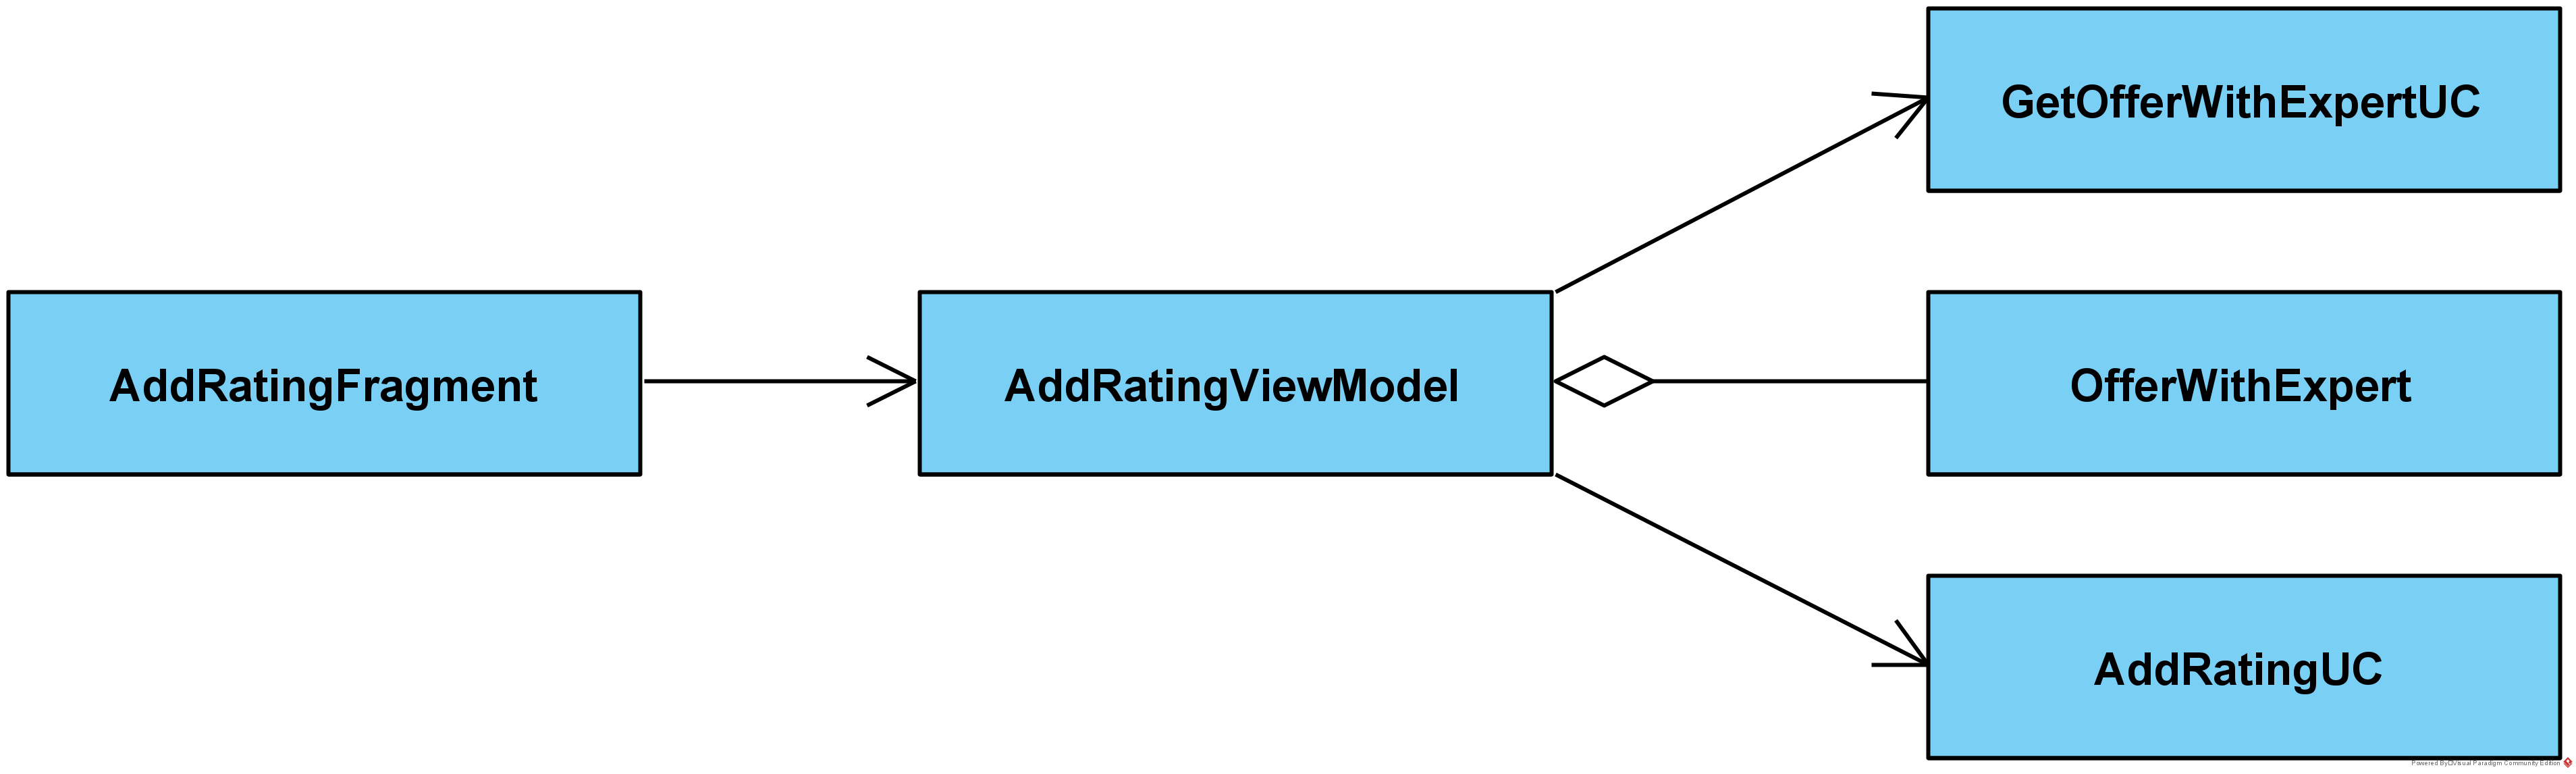
\includegraphics[width=\linewidth]{images/mvvm_example.png}
%   \caption{Wzorzec MVVM na przykładzie dodawania oceny}
%   \label{fig:mvvm-example}
% \end{figure}

% Na rysunku \ref{fig:mvvm-example} przedstawione zostało wykorzystanie wzorca MVVM na przykładzie dodawania oceny przez klienta. Klasa AddRatingViewModel stanowi ViewModel i zaczyna od wykonania przypadek użycia GetOfferWithExpertUC by dostać obiekt domenowy OfferWithExpert reprezentujący ofertę i wykonawcę, którego ma dotyczyć dodawana ocena. Zaktualizowanie tych wartości jest zauważane przez widok dzięki mechanizmowi subskrypcji i aktualizuje on natychmiastowo swoją zawartość. Gdy użytkownik uzupełni już ocenę i wciśnie przycisk potwierdzenia to widok poinformuje o tym ViewModel poprzez wywołanie jego odpowiedniej metody, który wykona przypadek użycia AddRatingUC i ocena zostanie dodana.

\section{Warstwa danych}
\label{wzorzec-repozytorium}

% Warstwa danych została zaimplementowana jako zbiór jedenastu repozytoriów. Stanowią one sposób na zapewnienie abstrakcji dostępu do danych i wszelkie operacje na danych mogą być wykonywane jedynie za ich pomocą. Zapewnia to spójność aplikacji i łatwość wprowadzania ewentualnych zmian w sposobie przechowywania informacji. Wszystkie repozytoria wraz z metodami, które posiadają, zostały przedstawione w postaci diagramu na rysunku \ref{fig:repos}.

Warstwa danych została zaimplementowana jako zbiór jedenastu repozytoriów, które stanowią sposób na zapewnienie abstrakcji dostępu do informacji. Umożliwia to dokonywanie zmian w sposobie przechowywania danych bez wpływu na logikę, która z nich korzysta.
Wszelkie operacje odczytu i modyfikacji wykonywane są jedynie za ich pomocą. Oznacza to, że pełnią rolę pojedynczego źródła prawdy (ang. Single Source of Truth). Zapewnia to spójność wyświetlanych przez aplikację informacji. Wszystkie repozytoria wraz z metodami, które posiadają, zostały przedstawione w postaci diagramu na rysunku \ref{fig:repos}.

\begin{figure}[ht!]
  \centering
  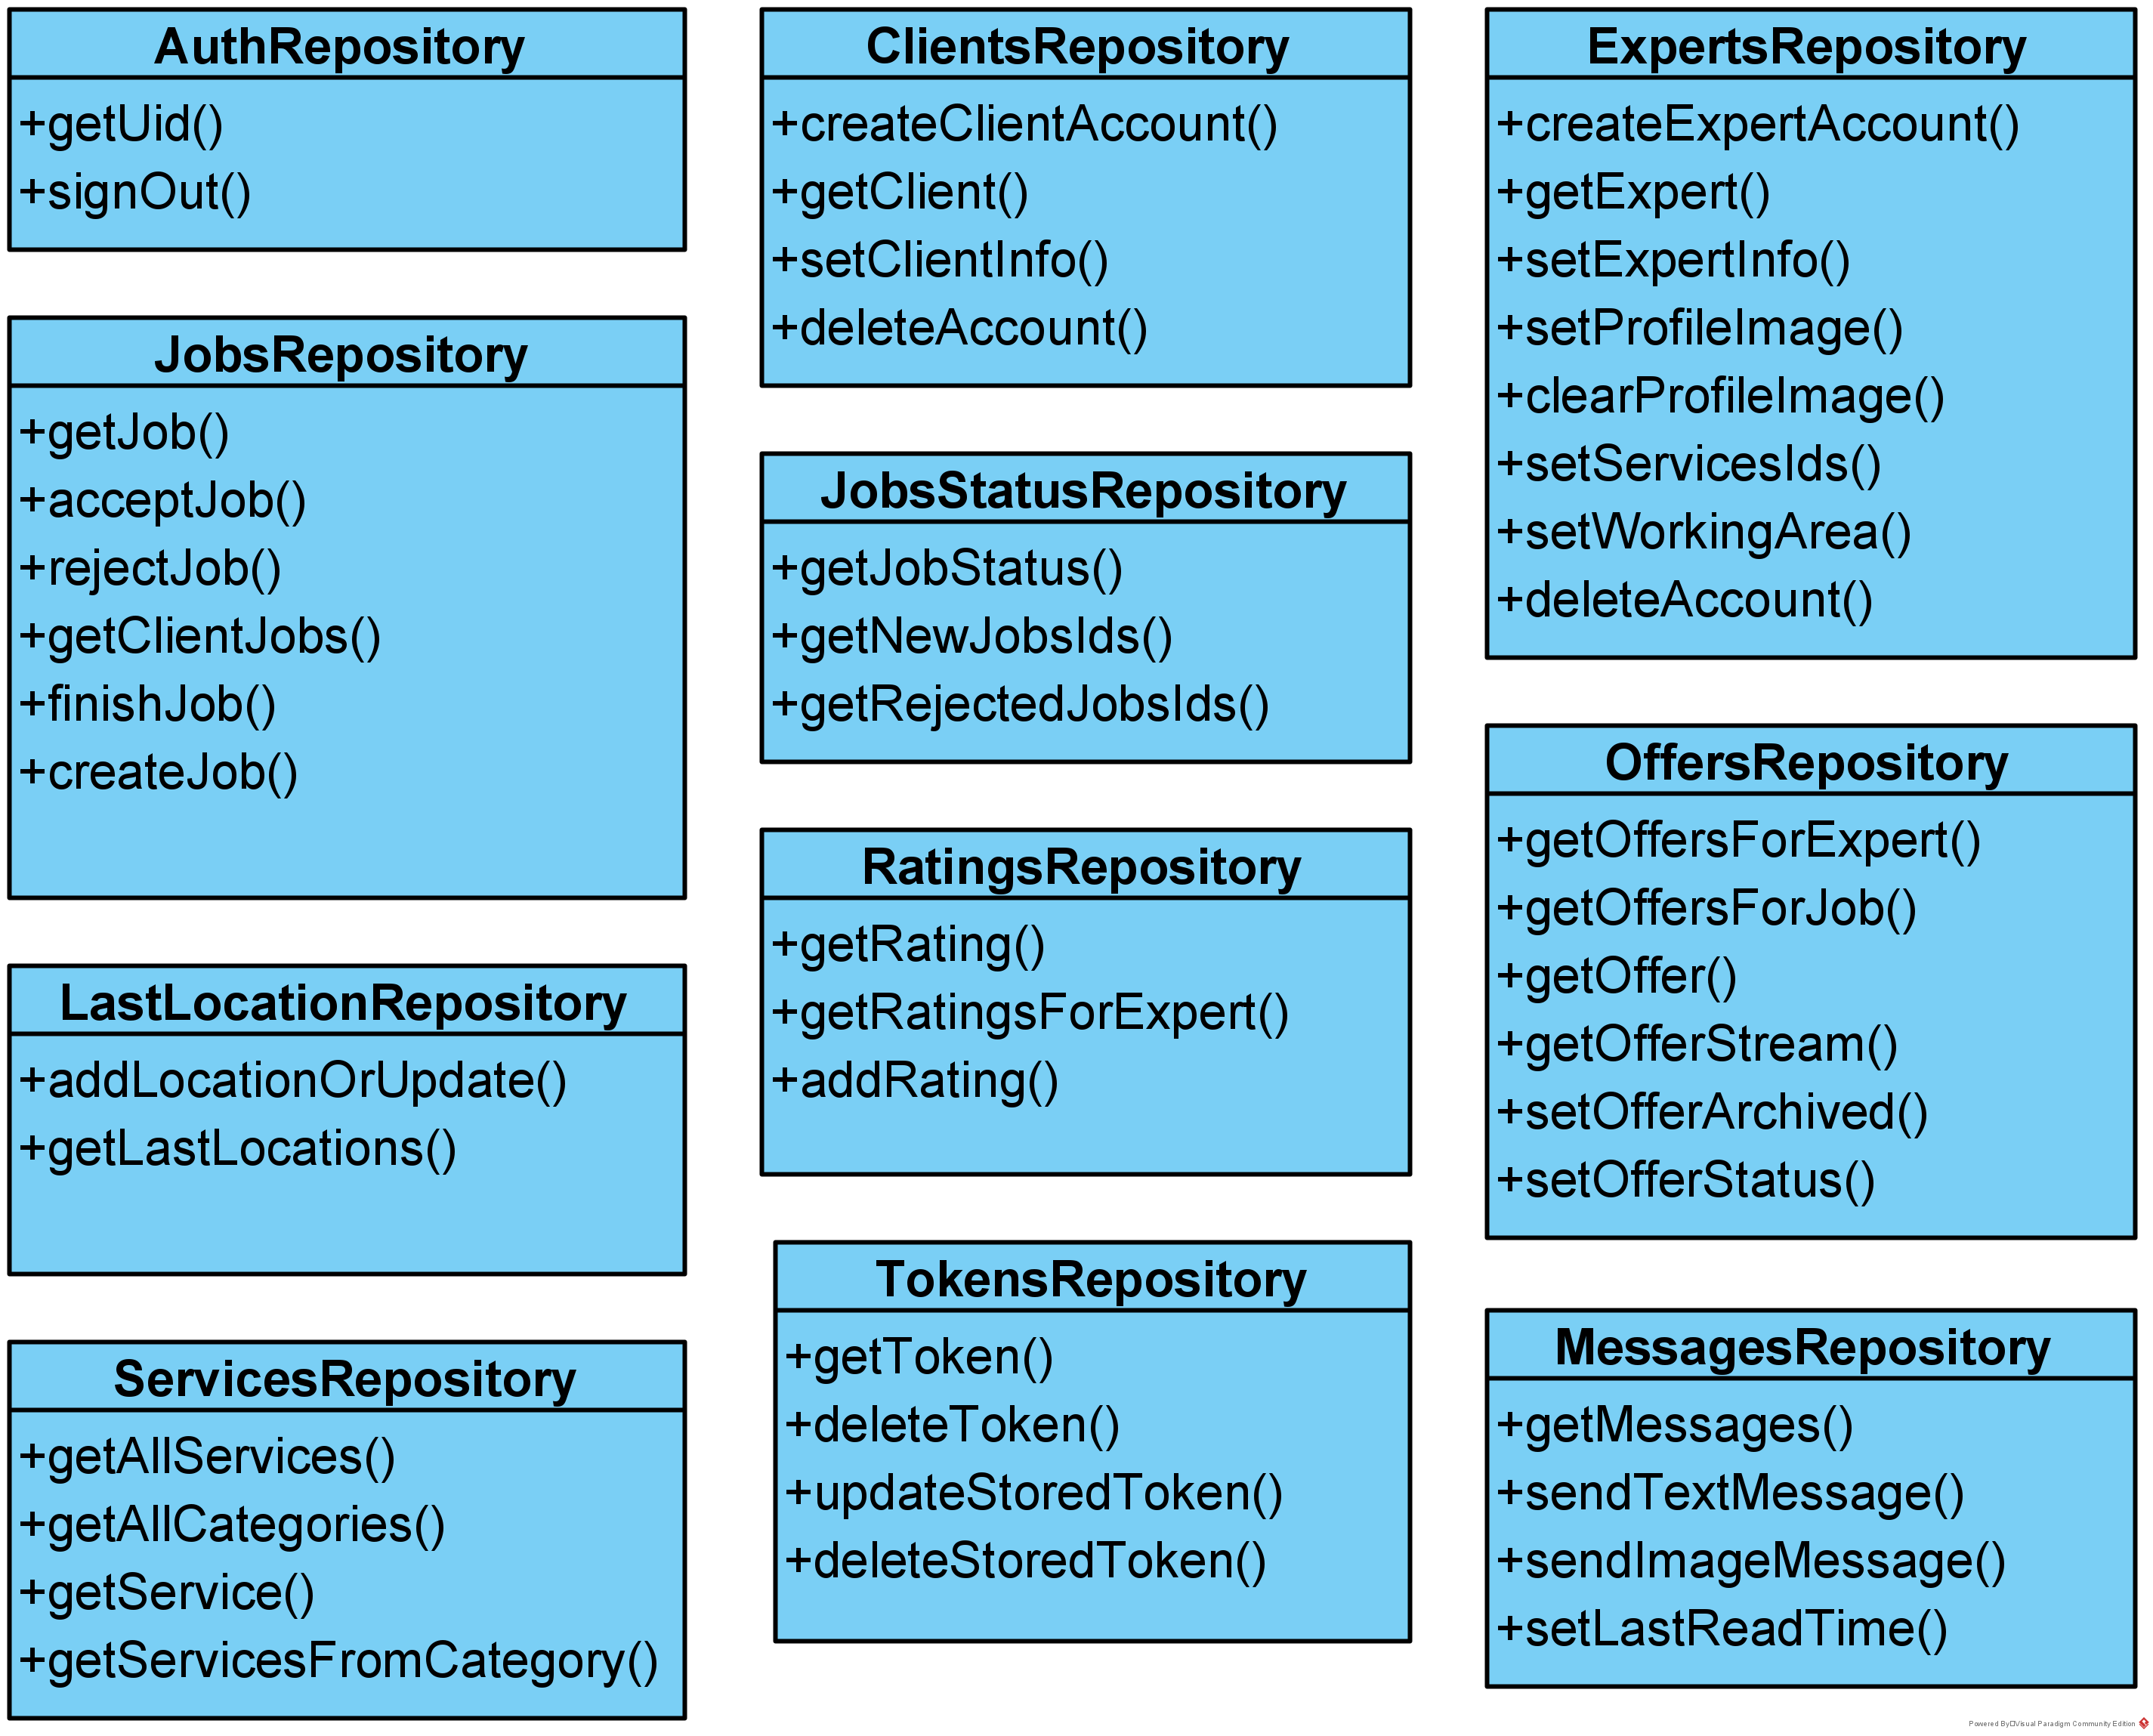
\includegraphics[width=\linewidth]{images/repositories.png}
  \caption{Diagram UML klas repozytoriów}
  \label{fig:repos}
\end{figure}

Każde repozytorium zostało stworzone z myślą o zarządzaniu konkretnym typem danych. Są one następujące:
\begin{itemize}
    \item \textbf{\code{AuthRepository}} - dane autoryzacji;
    \item \textbf{\code{ClientsRepository}} - klienci;
    \item \textbf{\code{ExpertsRepository}} - wykonawcy;
    \item \textbf{\code{JobsRepository}} - zlecenia;
    \item \textbf{\code{JobsStatusRepository}} - statusy zleceń, czyli informacje o ich dostępności z punktu widzenia konkretnych wykonawców;
    \item \textbf{\code{LastLocationsRepository}} - ostatnio użyte podczas dodawania zleceń lokalizacje;
    \item \textbf{\code{RatingsRepository}} - oceny wystawiane przez klientów;
    \item \textbf{\code{OffersRepository}} - oferty;
    \item \textbf{\code{ServicesRepository}} - usługi oraz kategorie usług;
    \item \textbf{\code{TokensRepository}} - tokeny FCM, wykorzystywane do notyfikacji push;
    \item \textbf{\code{MessagesRepository}} - wiadomości z chatu.
\end{itemize}

Wewnętrznie, aby wykonywać swoje zadania, repozytoria wykorzystują źródła danych. W aplikacji przewidziane zostały dwa źródła: lokalna baza danych ROOM oraz Firebase, przez który rozumiane są wszystkie dostępne w jego ramach usługi. Zostało to przedstawione na rysunku \ref{fig:data-sources}.

\begin{figure}[ht]
  \centering
  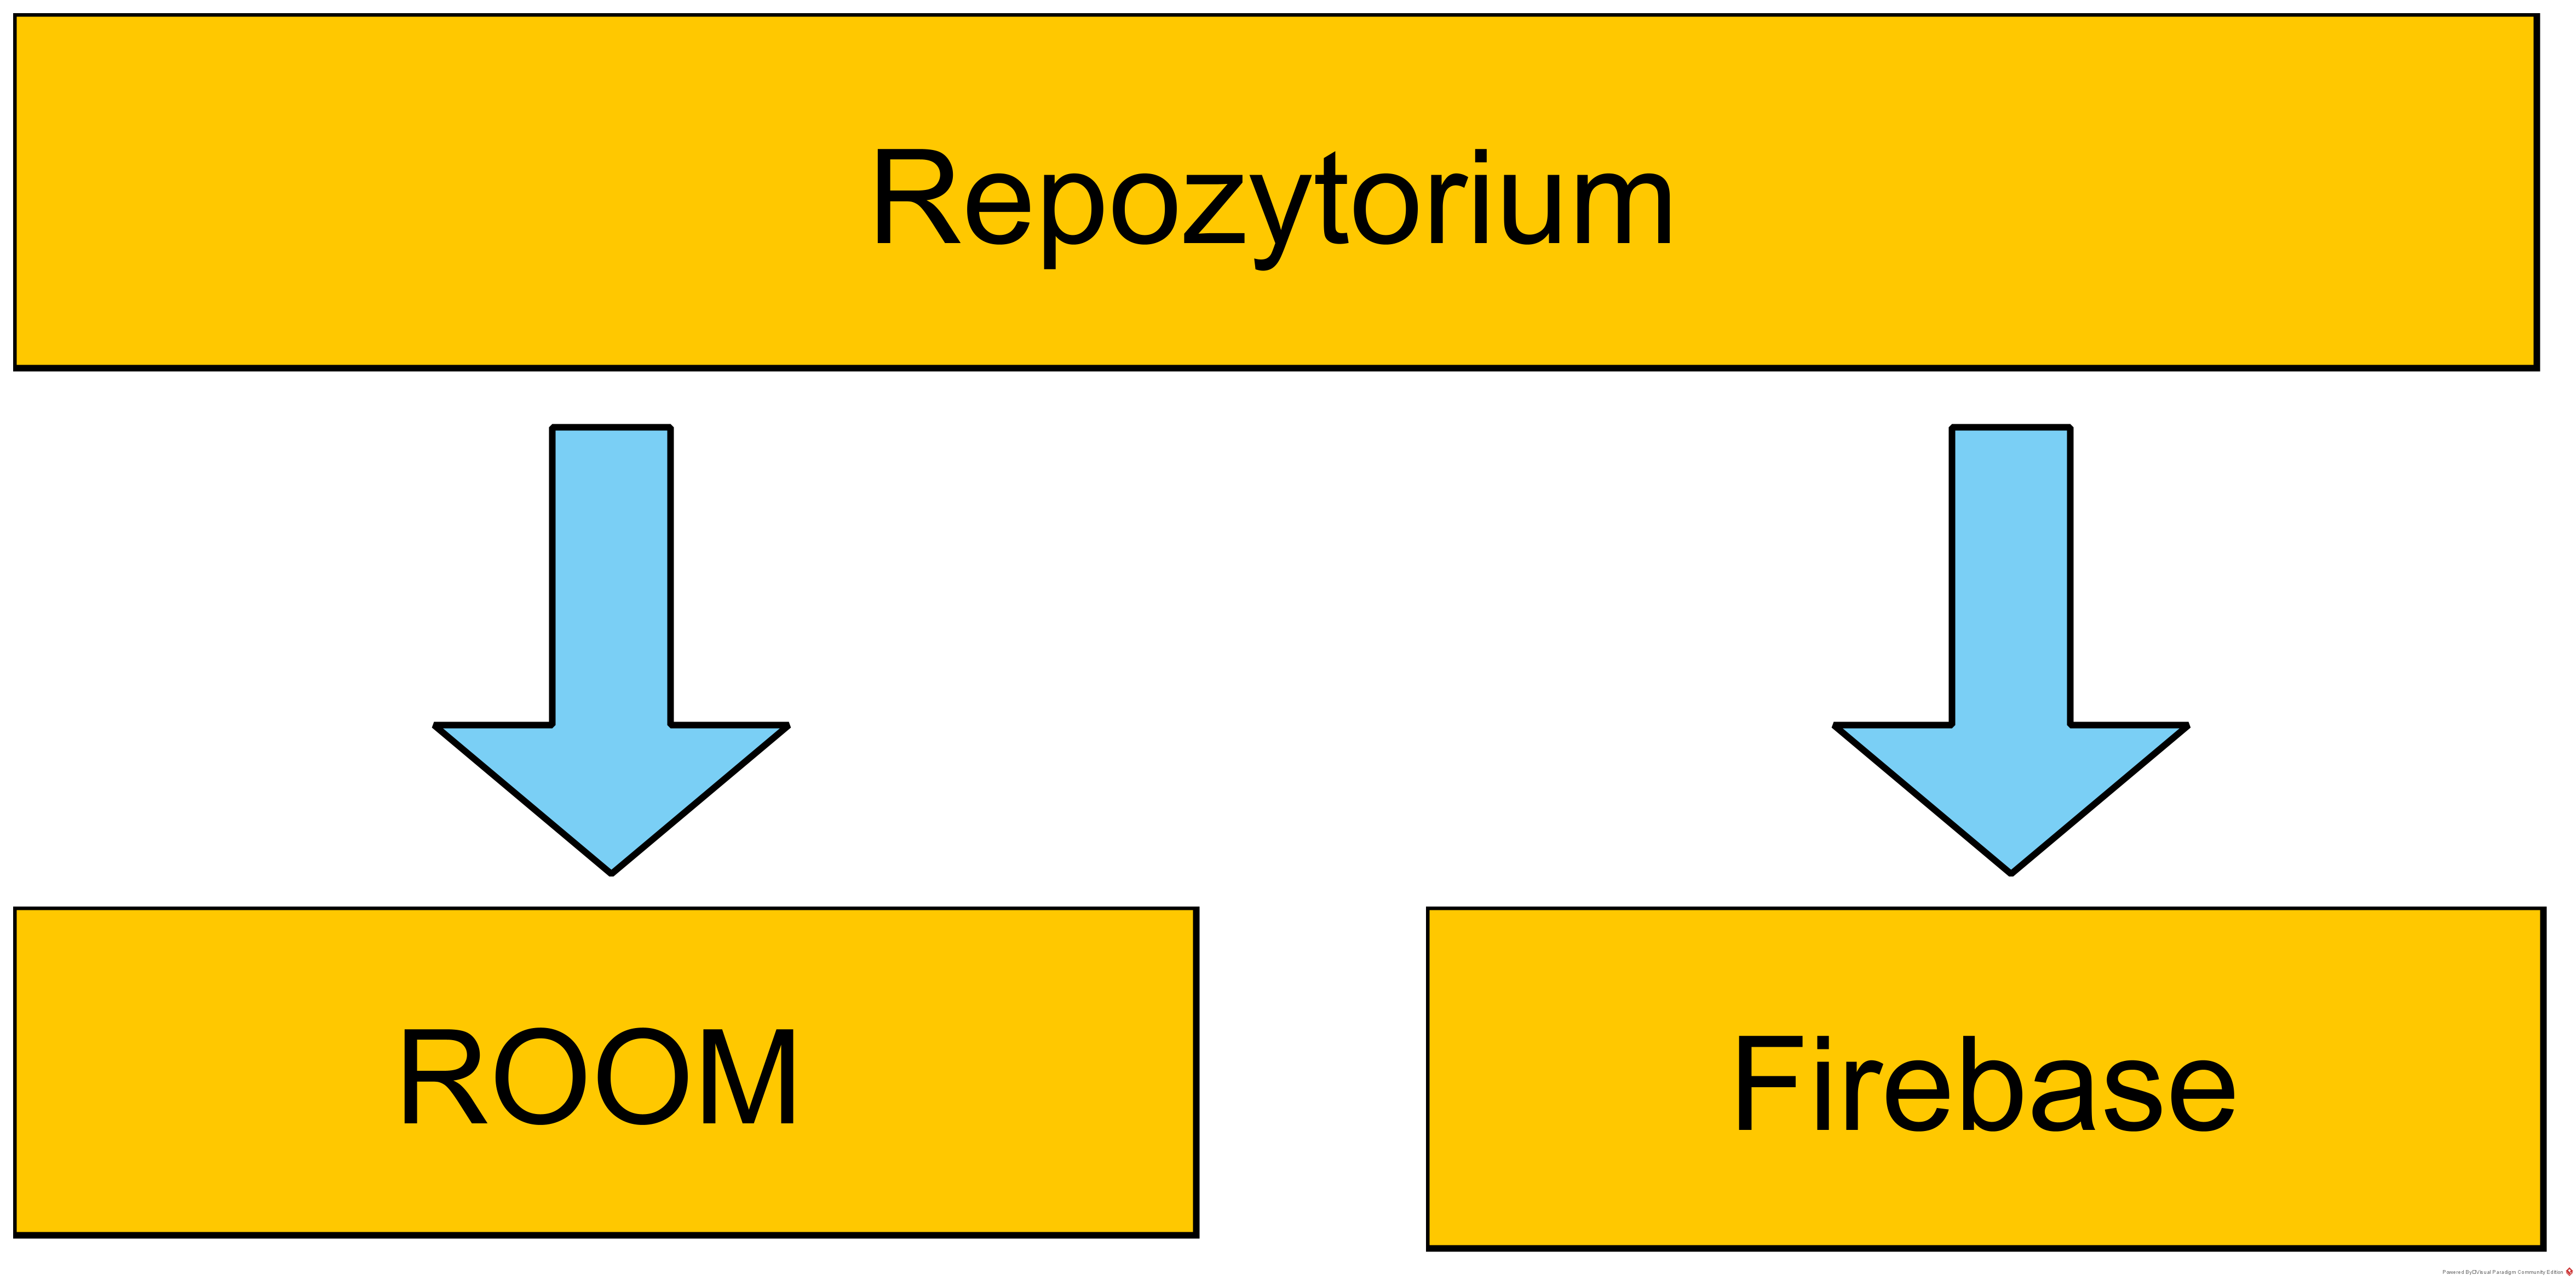
\includegraphics[width=0.7\linewidth]{images/data_sources.png}
  \caption{Schemat wykorzystania źródeł danych przez repozytoria}
  \label{fig:data-sources}
\end{figure}

W zależności od potrzeby repozytoria wykorzystują jedno lub oba źródła danych. Repozytorium \code{LastLocationsRepository}, zarządzające ostatnio wybieranymi lokalizacjami, wymaga jedynie lokalnej bazy ROOM, ponieważ są to informację, które mogą być zapisywane tylko lokalnie, a ich przechowywanie w zdalnej bazie danych jest zbędne. Repozytorium \code{MessagesRepository} wykorzystuje z kolei jedynie Firebase, ponieważ wiadomości z chatu muszą być dodawane i pobierane ze zdalnej bazy danych, by mogły być współdzielone pomiędzy użytkownikami. Korzystanie z bazy ROOM nie jest tutaj dodatkowo potrzebne, ponieważ używana baza Firebase Firestore posiada wbudowany mechanizm cachowania. Repozytorium \code{JobsStatusRepository} potrzebuje już jednak obu źródeł danych, ponieważ statusy zleceń są pobierane z Firebase przy pomocy funkcji Firebase Functions, które nie posiadają wbudowanego cachowania i pożądane jest wykorzystanie również lokalnej bazy danych ROOM, by je zapewnić.

\section{Współdzielenie kodu}
\label{code-sharing}

Na szczególną uwagę zasługują rozwiązania, które wykorzystano w celu minimalizacji duplikacji kodu pomiędzy aplikacjami dla klientów oraz wykonawców. Obie zawierają bowiem często podobne ekrany, które różnią się pewnymi zachowaniami, kolorami lub innymi nielicznymi elementami. 

O potrzebie unikania powtórzeń w kodzie mówi stosowana przez programistów reguła DRY (ang. Don't Repeat Yourself), która została sformułowana przez Andy'ego Hunta oraz Dave'a Thomasa w książce \enquote{Pragmatyczny programista} \cite{pragmatic-programmer}. Pomaga ona uniknąć błędów powstających podczas wielokrotnego wykonywania tej samej czynności oraz oszczędza czas.

Podstawowym działaniem jakie poczyniono w kierunku uniknięcia duplikacji kodu jest podział na trzy moduły, które zostały przedstawione na rysunku \ref{fig:moduły}. Moduły client oraz expert to moduły aplikacji. Są one zależne od moduł common, który jest modułem bibliotecznym, w którym zdecydowano się umieszczać współdzielony kod. 

\begin{figure}[ht!]
  \centering
  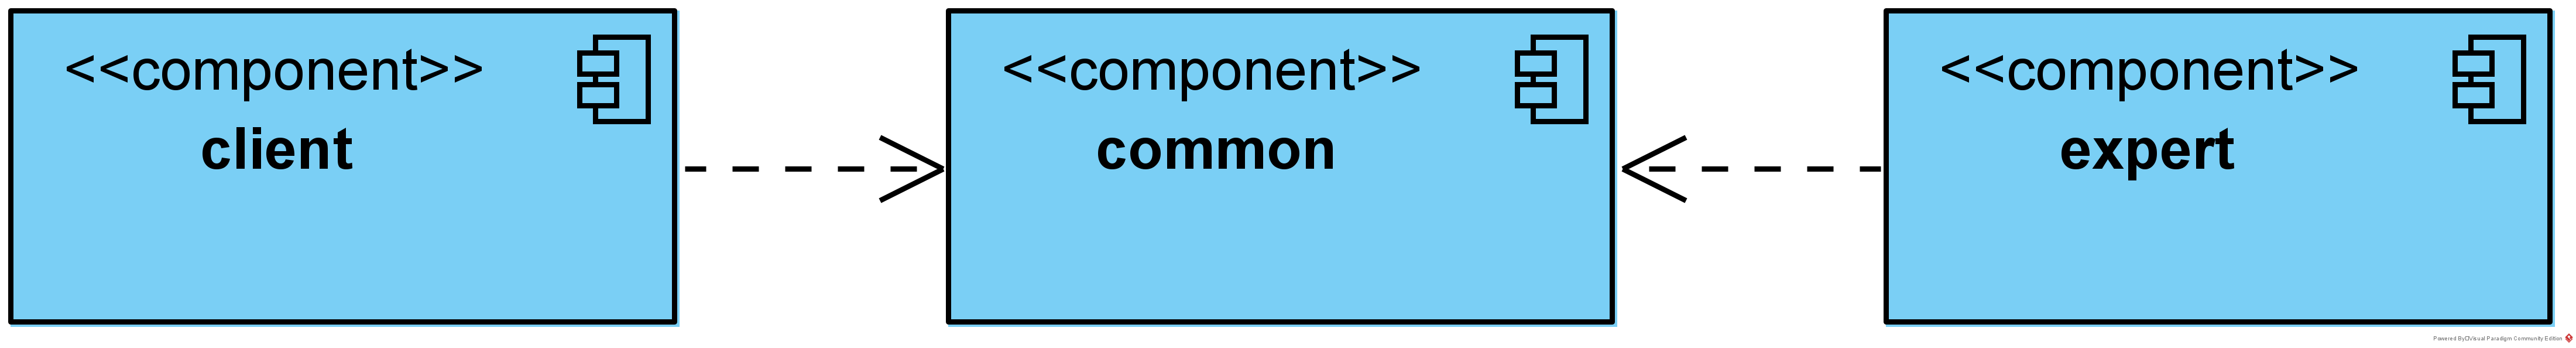
\includegraphics[width=\linewidth]{images/modules.png}
  \caption{Diagram UML przedstawiający stworzone moduły i ich relacje}
  \label{fig:moduły}
\end{figure}

W module common zostały umieszczone między innymi wszystkie repozytoria składające się na warstwę danych oraz wszystkie modele domenowe, ponieważ są to elementy, które w zdecydowanej większości są wykorzystywane w obu aplikacjach. Niektóre z nich są w rzeczywistości potrzebne tylko w jednej, lecz takich elementów jest na tyle mało, że zdecydowano się ich nie rozdzielać w celu utrzymania prostoty.

Na rysunku \ref{fig:dziedziczenie} przedstawiony został diagram UML przedstawiający sposób wykorzystania tych modułów na przykładzie ekranów usuwania konta klienta i wykonawcy. Ekrany te są do siebie wyraźnie podobne, różnią się jedynie kolorami, treścią wyświetlanych wiadomości oraz usuwaniem różnych obiektów.

\begin{figure}[ht!]
  \centering
  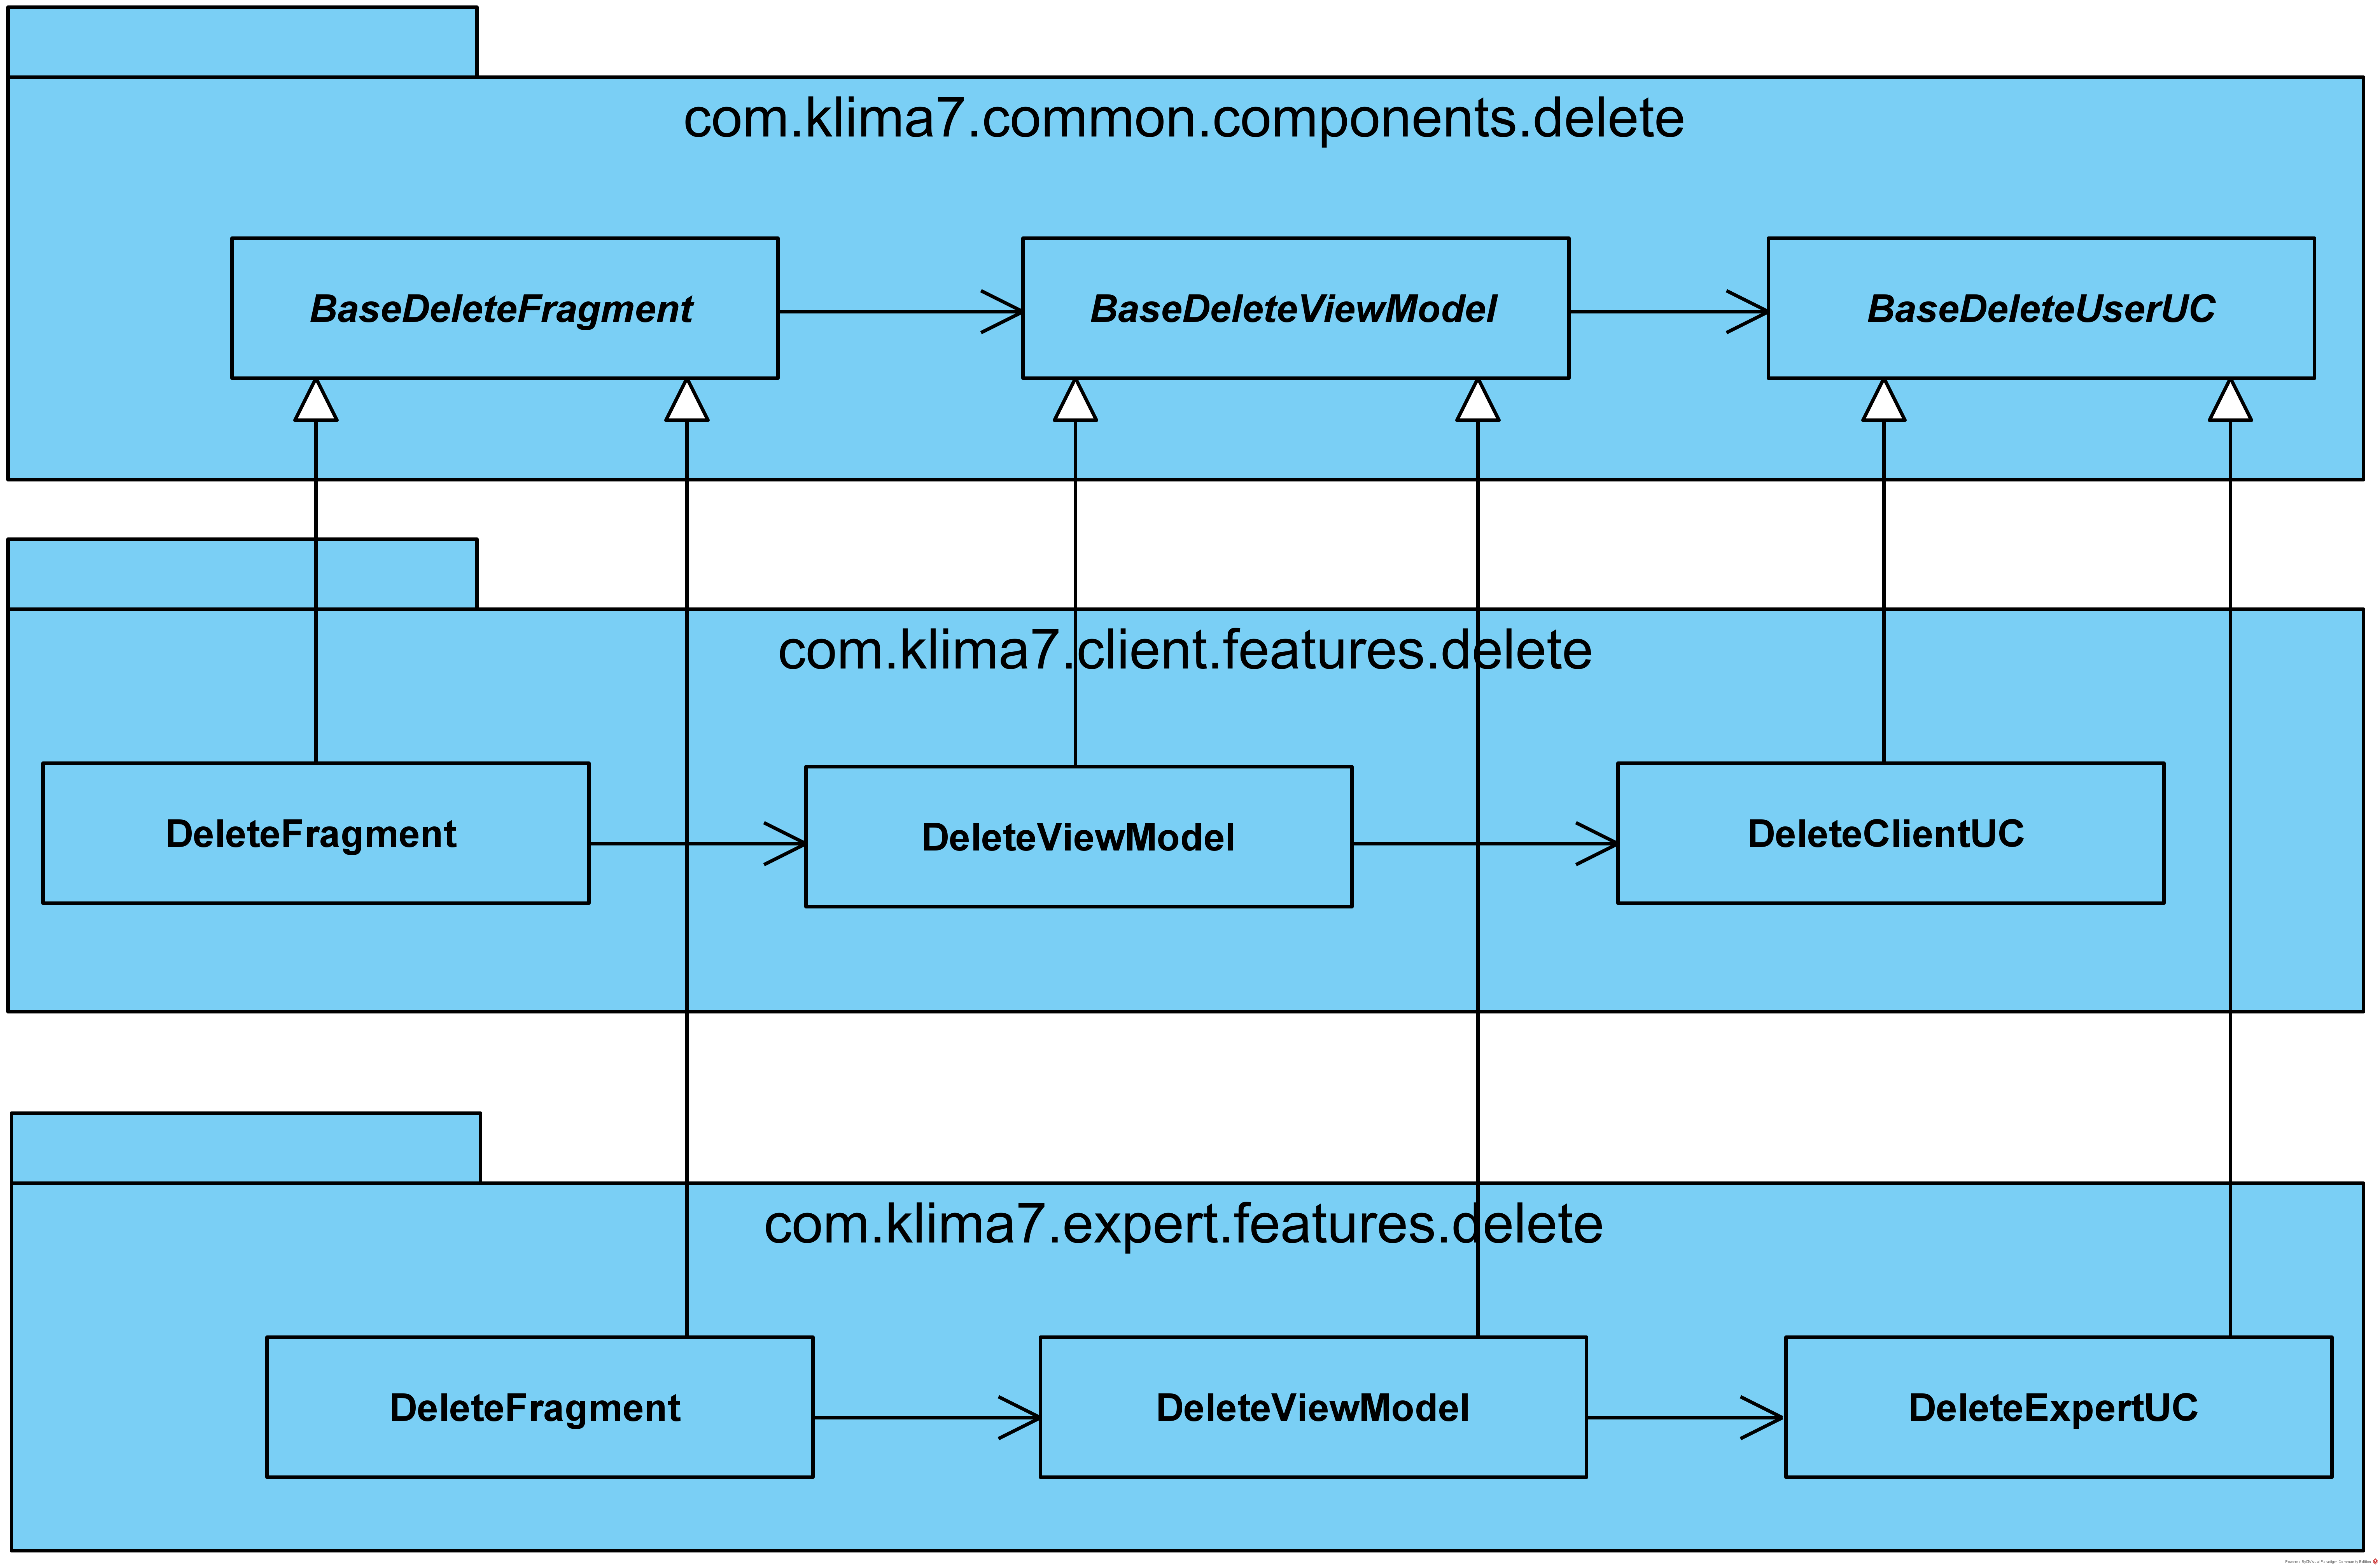
\includegraphics[width=\linewidth]{images/modules_example.png}
  \caption[Diagram UML prezentujący wykorzystanie modułów na przykładzie]{Diagram UML prezentujący wykorzystanie modułów dla współdzielenia kodu na przykładzie ekranów usuwania użytkowników}
  \label{fig:dziedziczenie}
\end{figure}

W celu zaimplementowania ekranów usuwania w module common zostały stworzone klasy bazowe. \code{BaseDeleteFragment} stanowi widok, \code{BaseDeleteViewModel} stanowi ViewModel, a \code{BaseDeleteUserUC} jest przypadkiem użycia usuwającym użytkownika. Są to jednak klasy abstrakcyjnie, co widać na diagramie UML po pochylonej czcionce. Oznacza to, że nie można ich bezpośrednio wykorzystać i konieczne jest ich rozszerzenie, co ma miejsce w modułach client oraz expert, gdzie podczas dziedziczenia dodawany jest do nich specyficzny dla danej aplikacji kod. W podobny sposób zostały zrealizowane również inne ekrany, które występują w dwóch alternatywnych wersjach.